\documentclass[11pt]{article} 
\addtolength{\hoffset}{-2.25cm}
\addtolength{\textwidth}{4.5cm}
\addtolength{\voffset}{-3.25cm}
\addtolength{\textheight}{5cm}
\setlength{\parskip}{0pt}
\setlength{\parindent}{0in}
\usepackage{tabularx}

\usepackage{algorithm}
\usepackage{listings}
\usepackage{empheq}
\usepackage[noend]{algpseudocode}
\newcommand{\algrule}[1][.2pt]{\par\vskip.5\baselineskip\hrule height #1\par\vskip.5\baselineskip}

\usepackage{blindtext} % Package to generate dummy text
\usepackage{charter} % Use the Charter font
\usepackage[shortlabels]{enumitem} %for enum purpose
\usepackage[utf8]{inputenc} % Use UTF-8 encoding

\usepackage[english]{babel} % Language hyphenation and typographical rules
\usepackage{amsthm, amsmath, amssymb} % Mathematical typesetting
\usepackage{float} % Improved interface for floating objects
\usepackage[final, colorlinks = true, 
            linkcolor = black, 
            citecolor = black]{hyperref} % For hyperlinks in the PDF
\usepackage{graphicx, multicol} % Enhanced support for graphics
\usepackage{xcolor} % Driver-independent color extensions
\usepackage{marvosym, wasysym} % More symbols
\usepackage{rotating} % Rotation tools
\usepackage{censor} % Facilities for controlling restricted text
\usepackage{hyperref}
\hypersetup{
    colorlinks=true,
    linkcolor=blue,
    filecolor=magenta,      
    urlcolor=black,
    }
    
\begin{document}

%-------------------------------
%	TITLE SECTION
%-------------------------------

\title{\centering{\textbf{COL352 \\ Introduction to Automata and Theory of Computation \\ Problem Set 3 }}}
\author{{\small{Swaraj Gawande (2019CS10406), Nishant Kumar (2019CS50586), Gaurav Jain (2019CS10349)}}}
\date{}
%-------------------------------
%	CONTENTS
%-------------------------------

\maketitle

\begin{enumerate}

    \algrule
    
    \item We say that a context-free grammar G is self-referential if for some non-terminal symbol $X$ we have $X \to^* \alpha X \beta$, where $\alpha, \beta \neq \varepsilon$. Show that a CFG that is not self-referential is regular.
    
    \textbf{Solution:}
    
    Let $G = (V,T,P,S)$ be a non self-referential context-free grammar. Define a directed graph $g$ in which the nodes are non-terminals/variables ($V$) and the edges are production rules. Suppose $A \rightarrow \alpha B \beta$ is a production rule and $\alpha, \beta \in (V \cup T)^* \cup \{ \epsilon \}$ then there is an edge from non-terminal $A$ to non-terminal $B$. \\
    The graph $g$ can be separated into strongly-connected components. Suppose the strongly-connected components of $g$ are $S_1, S_2, S_3, ... , S_n$ sorted in some topological order.
    
    \textbf{Claim:} $S_i$ contains production rules of type ($A \rightarrow \alpha$ and $A \rightarrow B \alpha$) where $\alpha \in T$ (Left linear grammar) or ($A \rightarrow \alpha$ and $A \rightarrow \alpha B$) where $\alpha \in T$ (Right linear grammar).
    
    \textbf{Proof:} Proof by Contradiction. Suppose $S_i$ contains both a left linear rule say, $A \rightarrow \alpha B$ and a right linear rule say, $C \rightarrow D \beta$. Since $S_i$ is strongly-connected so there must be a path from $B$ to $C$ and $D$ to $A$. So, $A \rightarrow \alpha B \rightarrow^* \alpha \gamma C \delta \rightarrow \alpha \gamma D \beta \delta \rightarrow^* \alpha \gamma \gamma' A \delta' \beta \delta $. Here, $\alpha$ and $\beta$ should be non-empty. This is a contradiction to the non self-referential property of the given grammar as there is a self-referential derivation for non-terminal $A$. 
    
    Since each strongly-connected component has either only left linear production rules or right linear production rules. We can use the famous result that all left-linear or right-linear grammars are regular languages. Thus, for each strongly-connected component $S_i$, we can construct its corresponding NFA $N_i$.
    
    We construct a NFA $N$ which accepts the language $L(G)$ using the NFAs $N_i$. To transition between NFA $N_{i-1}$ and $N_i$, we modify the production rules of $N_{i-1}$ to point to the NFA $N_i$. This NFA $N$ can accept $L(G)$ by moving through NFAs $N_i$ and accepted in some NFA $N_j$. 
    
    Hence, G which is non referential context-free grammar is regular. \hfill\qedsymbol
    
    \algrule
    \clearpage
    \item Prove that the class of context-free languages is closed under intersection with regular languages. That is, prove that if $L_1$ is a context-free language and $L_2$ is a regular language, then $L_1 \cap L_2$ is a context-free language. Do this by starting with a DF.

    \textbf{Solution:} 
    
    Given $L_1$ is context free language whereas language $L_2$ is regular language.\\
    Let $A=(Q_A,\Sigma,\Gamma,\delta_A,q_{0_A},\perp,F_A)$ be the push down automata accepting language $L_1$ and $N=(Q_N,\Sigma,\delta_N,q_{0_N},F_N)$ be the DFA accepting the language $L_2$.\\
    We can now construct an PDA $B=(Q_B,\Sigma,\Gamma,\delta_B,q_{0_B},\perp,F_B)$ where $Q_B=Q_AxQ_N$, $q_{0_B}=(q_{0_A},q_{0_N})$ and $F_B=F_A \times F_N$ such that it simulates the PDA $A$ and the NFA $N$ running together i.e. the the transitions $\delta"$ from a general state $(q_a,q_n)$ on reading character $c$ with stack head is stack character $s$ would be- 
    \begin{center}
        $\delta((q_a,q_n),c,S)=(((q_a',q_n'),S')\ |\ q_a'=\delta_N(q_a,c)$ and $(q_n',S')=\delta_A(q_a,c,S))$
    \end{center}
    Where as epsilon transitions are of the form-
    \begin{center}
        $\delta((q_a,q_n),\epsilon,S)=(((q_a,q_n'),S')\ |\ (q_n',S')=\delta_A(q_a,c,S))$
    \end{center}
    \textbf{Claim:} The PDA $B$ constructed above accepts the language $L_3=L_1\cap L_2$ i.e.$L_3$ is context free language.
    
    \textbf{Proof:} For a word $w$ in language $L_3$ there exists a run on PDA B such that-
    \begin{center}
        $(q_{0_B},w,\perp)\vdash^*(q_f,\in\gamma)\ |\ q_f\  \epsilon\  F_B$.
    \end{center}
    \textit{Proof by induction}\\
    Base case for empty string read, both the PDA A and DFA N are at initial state and so is our new DFA B. \\
    Consider a run of PDA A and DFA N on the word w of the form xy where string x is already read whereas string y is yet to be read. The PDA B is is a state $((q_a,q_n),S)$ and $q_n$ is the state at which DFA N would be after reading string x where as $q_a$ is the state at which PDA A is after reading string x and has stack in state $S$. Consider a transition now $\delta((q_a,q_n),c,s)$ if $c=\epsilon$ i.e we do not read a new character from the word the DFA  remains at the same state while the PDA might change its stack state from $S$ to $S'$ and its state from $q_a$ to $q_a'$ which is done by transition in PDA B to state $((q_a,q_n'),S')$. \\
    Whereas after reading another character the DFA N's state changes accordingly as well and result into the transition to state $((q_a',q_n'),S')$. That is the PDA B is infact simulation of PDA A and DFA N running together and a word w is accepted only if it is accepted by the DFA N i.e. we reach a final state $q_{f_n}$ and is also accepted by PDA A i.e $(q_{0_A},w,\perp)\vdash^*(q_{f_a},\epsilon,\gamma)\ |\ q_{f_a}\epsilon\ F_A$ which corresponds to PDA B ending at final state $(q_{f_a},q_{f_n})$. If any of the DFA N or the PDA A does not accept the word w then the PDA B can never reach a final state in $F_AxF_N$.\\
    Now since we are able  to construct a valid PDA which accepts language $L_3=L_1\cap L_2$, $L_3$ turns out to be a context free language as well. \hfill\qedsymbol

    \algrule
        \clearpage
    \item Given two languages $L, L'$, denote by 
    $$L||L' := \{x_1y_1x_2y_2 \dots x_ny_n \mid x_1x_2 \dots x_n \in L, y_1y_2\dots y_n \in L'\}$$
    
    Show that if $L$ is a CFL and $L'$ is regular, then $L || L'$ is a CFL by constructing a PDA for $L || L'$. Is $L || L'$ a CFL if both $L$ and $L'$ are CFLs? Justify your answer.
	
	\textbf{Solution:}
	
	Let $P = (Q_1,\Sigma,\Gamma,\delta_1,q_1,\perp,F_1)$ be a NPDA such that $L = L(P)$. \\ Let $D = (Q_2,\Sigma,q_2,F_2,\delta_2)$ be a DFA such that $L' = L(D)$.\\
	Consider a NPDA $P' = (Q',\Sigma,\Gamma',\delta',q',\perp,F')$ where,\\
	$Q' = Q_1 \times Q_2$ \\
	$\Gamma' = \Gamma \cup \{X'\}$. $X'$ is a new stack alphabet.\\
 	$ q' = (q_1,q_2)$ \\
	$ F' = F_1 \times F_2$ \\
    $ \delta' ( (q_p,q_d), a, X ) =
	\begin{cases}
    ( ( q_p , \delta_2( q_d , a ) ) , \epsilon ) & \text{if}\ X = X' \\ 
	\{( ( q , q_d ) , X'\alpha )\ |\ (q,\alpha) \in \delta_1(q_p,a,X) \} & \text{if}\ X \neq X' 
	\end{cases}$ \\ \\
	We claim that this PDA $P'$ accepts the language $L||L'$ and thus, $L || L'$ is a context free language. We can prove the claim by observing that when the top alphabet in the stack is $X'$, there is a DFA transition corresponding to $q_d$, the state of the DFA $D$ and $a$, the character of the input string and the top stack alphabet is popped. When the top alphabet in the stack is not $X'$, then there is a PDA transition corresponding to $q_p$, the state of the PDA $P$ and $a$, the character of the input string and the top stack element is replaced by $X'\alpha$ where $\alpha$ is the stack alphabet string pushed by the PDA $P$. $X'$ is pushed on top of $\alpha$.\\
	So, in a run of the PDA $P'$, first, there is a PDA transition and $X'$ is pushed on top of stack. Now since the top is $X'$, there is a DFA transition corresponding to the input character. This process will continue and there will be PDA and DFA transitions alternatively. At the end of the run, if the PDA accepts the input sequence then it will reach a state $f_p \in F_1$ and similarly, DFA will reach a state $f_d \in F_2$. Thus, the PDA $P'$ accepts the input $w||w'$ if reaches $(f_p,f_d)$.\\
	Thus, $P'$ accepts $L||L'$ and hence, $L||L'$ is a context free language. \hfill\qedsymbol
	
    If both $L$ and $L'$ are CFLs then it is not necessary that $L||L'$ is also CFL. Consider the following case, let $L = \{ a^{2n} b^{n}\ |\ n > 0\}$ and 
    $L' = \{ a^{n} b^{2n}\ |\ n > 0\}$ then $L||L' = \{ a^{2n} (ab)^{n} b^{2n} \}$. $L$ and $L'$ are both context-free as they can easily be generated by the grammar $S \rightarrow aaSb\ |\ \epsilon$ and $S \rightarrow aSbb\ |\ \epsilon$ respectively. We can prove that $L||L'$ is not context-free using pumping lemma. Choose the pumping length to be p and $s = a^p b^{2p} c^p$. For all splits $s = uvwxy$, we can choose i=0 such that $uv^iwx^iy \notin L||L'$ as the composition of string will change as there is a $(ab)^n$ part in it which will disturb the structure of the string.
	
	
	\algrule
	\clearpage
	\item For $A \subseteq \Sigma^*$, define 
    $$cycle(A) = \{yx \mid xy \in A\}$$
    For example if $A = \{aaabc\}$, then 
    $$cycle(A) = \{aaabc, aabca, abcaa, bcaaa, caaab\}$$
    Show that if $A$ is a CFL then so is $cycle(A)$

		
	\textbf{Solution:} %Given a word $w$ of language $A$ to generate each word of $cycle(A)$ we can split $w$ as $xy$ then $yx \epsilon cycle(A)$.\\ Now for a given grammar $G$ in Chomsky Normal form to produce only such words $w \epsilon A$. We construct a new Grammar $G'$ such that for each production in $G$ of the form $A\longleftarrow BC$ where $B$ and $C$ are non-terminals there is a corresponding production $A\longleftarrow BC|B$ in $G'$ where as the productions of the form $A\longleftarrow \alpha$ where $\alpha$ is a terminal symbol are common to both $G$ and $G'$.The Grammar $G'$ thus produces all the prefixes possible, $x$, for the word $w$ in the language $A$. Which means the Language of prefixes $A_p$ is also a context free language. Now with similarly con
	
	For a word $w$ in language $A$ we need to show that if $w$ is of the form $xy$ then the language $cycle(A)$ containing all possible $yx$ for all words in $A$ is also a CFL. Now if $A$ is a CFL then say $P$ is the PDA accepting $A$. We would now construct a PDA $P'$ which would accept language $cycle(A)$. To do so we need to guess the end of string $y$ and then accept with appropriate string $x$. Now while reading string $y$ after reading string $x$ the stack may be non-empty and the PDA $P$ would need to pop these stack alphabets in process of reading $y$. In PDA $P'$ however we start with an empty stack and instead of popping we push the corresponding stack symbols to the stack at the transitions where $P$ would have popped those symbols.\\
	Now $P'$ non deterministically guesses the end of string $y$ and starts the acceptance of string $x$ by now popping the corresponding stack symbols in the stack of $P'$ in the same order in which they would have been pushed in the stack of $P$.\\
	\textbf{Claim:} The new PDA $P'$ thus constructed accepts language $cycle(A)$.\\
	\textbf{Proof:} While we are pushing the stack symbols while we were reading $y$ using $P'$. If the PDA guesses the end of string $y$ correctly then the stack would be just the reverse of what it would have been while after reading string $x$ using $P$ as those are the stack symbols which would be needed to be popped in reading $y$ using $P$ are already pushed in the stack of $P'$. Given the state of the the PDA and the state of the stack the string $x$ can be uniquely determined for a given $y$ such that $xy \in A$ and thus $yx$ is accepted. \hfill\qedsymbol
    
    \algrule
    \clearpage
    \item Let $$A = \{wtw^R\mid w,t, \in \{0,1\}^* \text{ \ and \ } |w| = |t|\}$$ Show that $A$ is not a CFL.
    
    \textbf{Solution:}
    
    \textit{Proof by Contradiction:}
    
    Assume $A$ is a CFL. Then, $A$ must follow Pumping Lemma for CFLs. For all $s = wtw^R \in A$, $|s|$ is a multiple of 3 as $|w| = |t| = |w^R|$.\\
    Let the pumping length be $p$. Choose $s = 1^{2p}0^p1^p1^{2p}$. Clearly, $s \in A$ and $|s| > p$. Then, by pumping lemma there exists $s = uvwxy$ such that $|vx| > 0$ and $|vwx| \leq p$.\\
    Consider the following cases on $vx$:
    
    
    \textbf{Case 1:} $|vx|$ is not a multiple of 3. In this case, $s' = uv^2wx^2y \notin A$ as the length of $s'$ is not a multiple of 3 and every string $s \in A$ must have length in multiples of 3.
    
    \textbf{Case 2:} $|vx| = 3r$ for some $r$.
    \begin{itemize}[]
    
        \item \textbf{Case 2.1:} $vwx$ lies in the last two thirds of $s$. Then, $s' = uv^2wx^2y \notin A$ as $s'$ contains 0s in its first third but not in the last third and we require the last third to be reverse of the first third which is not possible here.
        
        \item \textbf{Case 2.2:} Some part of $vwx$ is present in the first third of $s$. Since $|vwx| \leq p$ so, $vwx$ extends till the first half of the string $s$. This leads to the following subcases on $v$ and $x$:
            
            \begin{itemize}
                \item $v$ contains both 0 and 1. Then, $s' = uv^2wx^2y \notin A$ as $s'$ contains 0s in its first third but not in the last third and we require the last third to be reverse of the first third which is not possible here.
                
                \item $v$ is empty and $x$ contains 0 and in some cases 1 too. Then, $s' = uv^2wx^2y \notin A$ as $s'$ contains 0s in its first third (maybe in the second third) but not in the last third and we require the last third to be reverse of the first third which is not possible here.
                
                \item $v$ contains 1 or empty and x contains 1 or empty. Then, $s' = uv^{6p+1}wx^{6p}+1y \notin A$ as $s'$ contains 0 in the last third but not in the first third as the minimum length of $s'$ is $12p$ and 0s are present in the last $4p$ values. We require the last third to be reverse of the first third which is not possible here.
                
            \end{itemize}
        
        
        
    \end{itemize}
    
    Thus, for all cases we find a string $s' \notin A$. This is a contradiction to the pumping lemma. Hence, $A$ is not a CFL. \hfill\qedsymbol
    

    
    \algrule 
	\clearpage
	\item Prove the following stronger version of pumping lemma for CFLs: 
    If $A$ is a CFL, then there is a number $k$ where if $s$ is any string in $A$ of length at least $k$ then $s$ may be divided into five pieces $s = uvxyz$, satisfying the conditions:
    \begin{itemize}
        \item for each $i\geq 0$, $uv^ixy^iz \in A$
        \item $v \neq \varepsilon$, and $y \neq \varepsilon$, and
        \item $|vxy| \leq k$.
    \end{itemize}
	
	\textbf{Solution:}\\
    Let $G = (V,T,P,S_0)$ is the CFG accepting A. Let b be an upper bound on the size of the RHS of any production rule of G. Let us consider k to be $b^{2\vert V \vert + 1}$ and  $\vert s \vert \geq k$. The depth of the parse tree should be atleast $2\vert V \vert + 1$ as any parse tree of depth $2\vert V \vert + 1$ will have at most $b^{2\vert V \vert + 1}$ leaves.\\\\
    Let us consider parse tree T to be the smallest parse tree for s and depth of T $\geq$ $b^{2\vert V \vert + 1}$. By pigeon hole principle we can say that a non-terminal R have to repeat twice in the path of any parse tree having depth $\geq$ $\vert V \vert + 1$. So, for the parse tree T having depth $b^{2\vert V \vert + 1}$, a non-terminal R have to repeat at least thrice by pigeon hole principle.\\
    Figure 1 represents the parse tree of s and R is the non-terminal which is repeating thrice. If we replace the sub-tree t with the sub-tree with last R as root we will get parse tree shown in Figure 2 which represents the string uxz. If we extend the the parse tree T as shown in Figure 3 we will get string $uv^2xy^2z$. So, with similar construction we can show for each $i \geq 0$, $uv^ixy^iz \in A$
    
    \begin{figure*}[!htb]
    \centering
    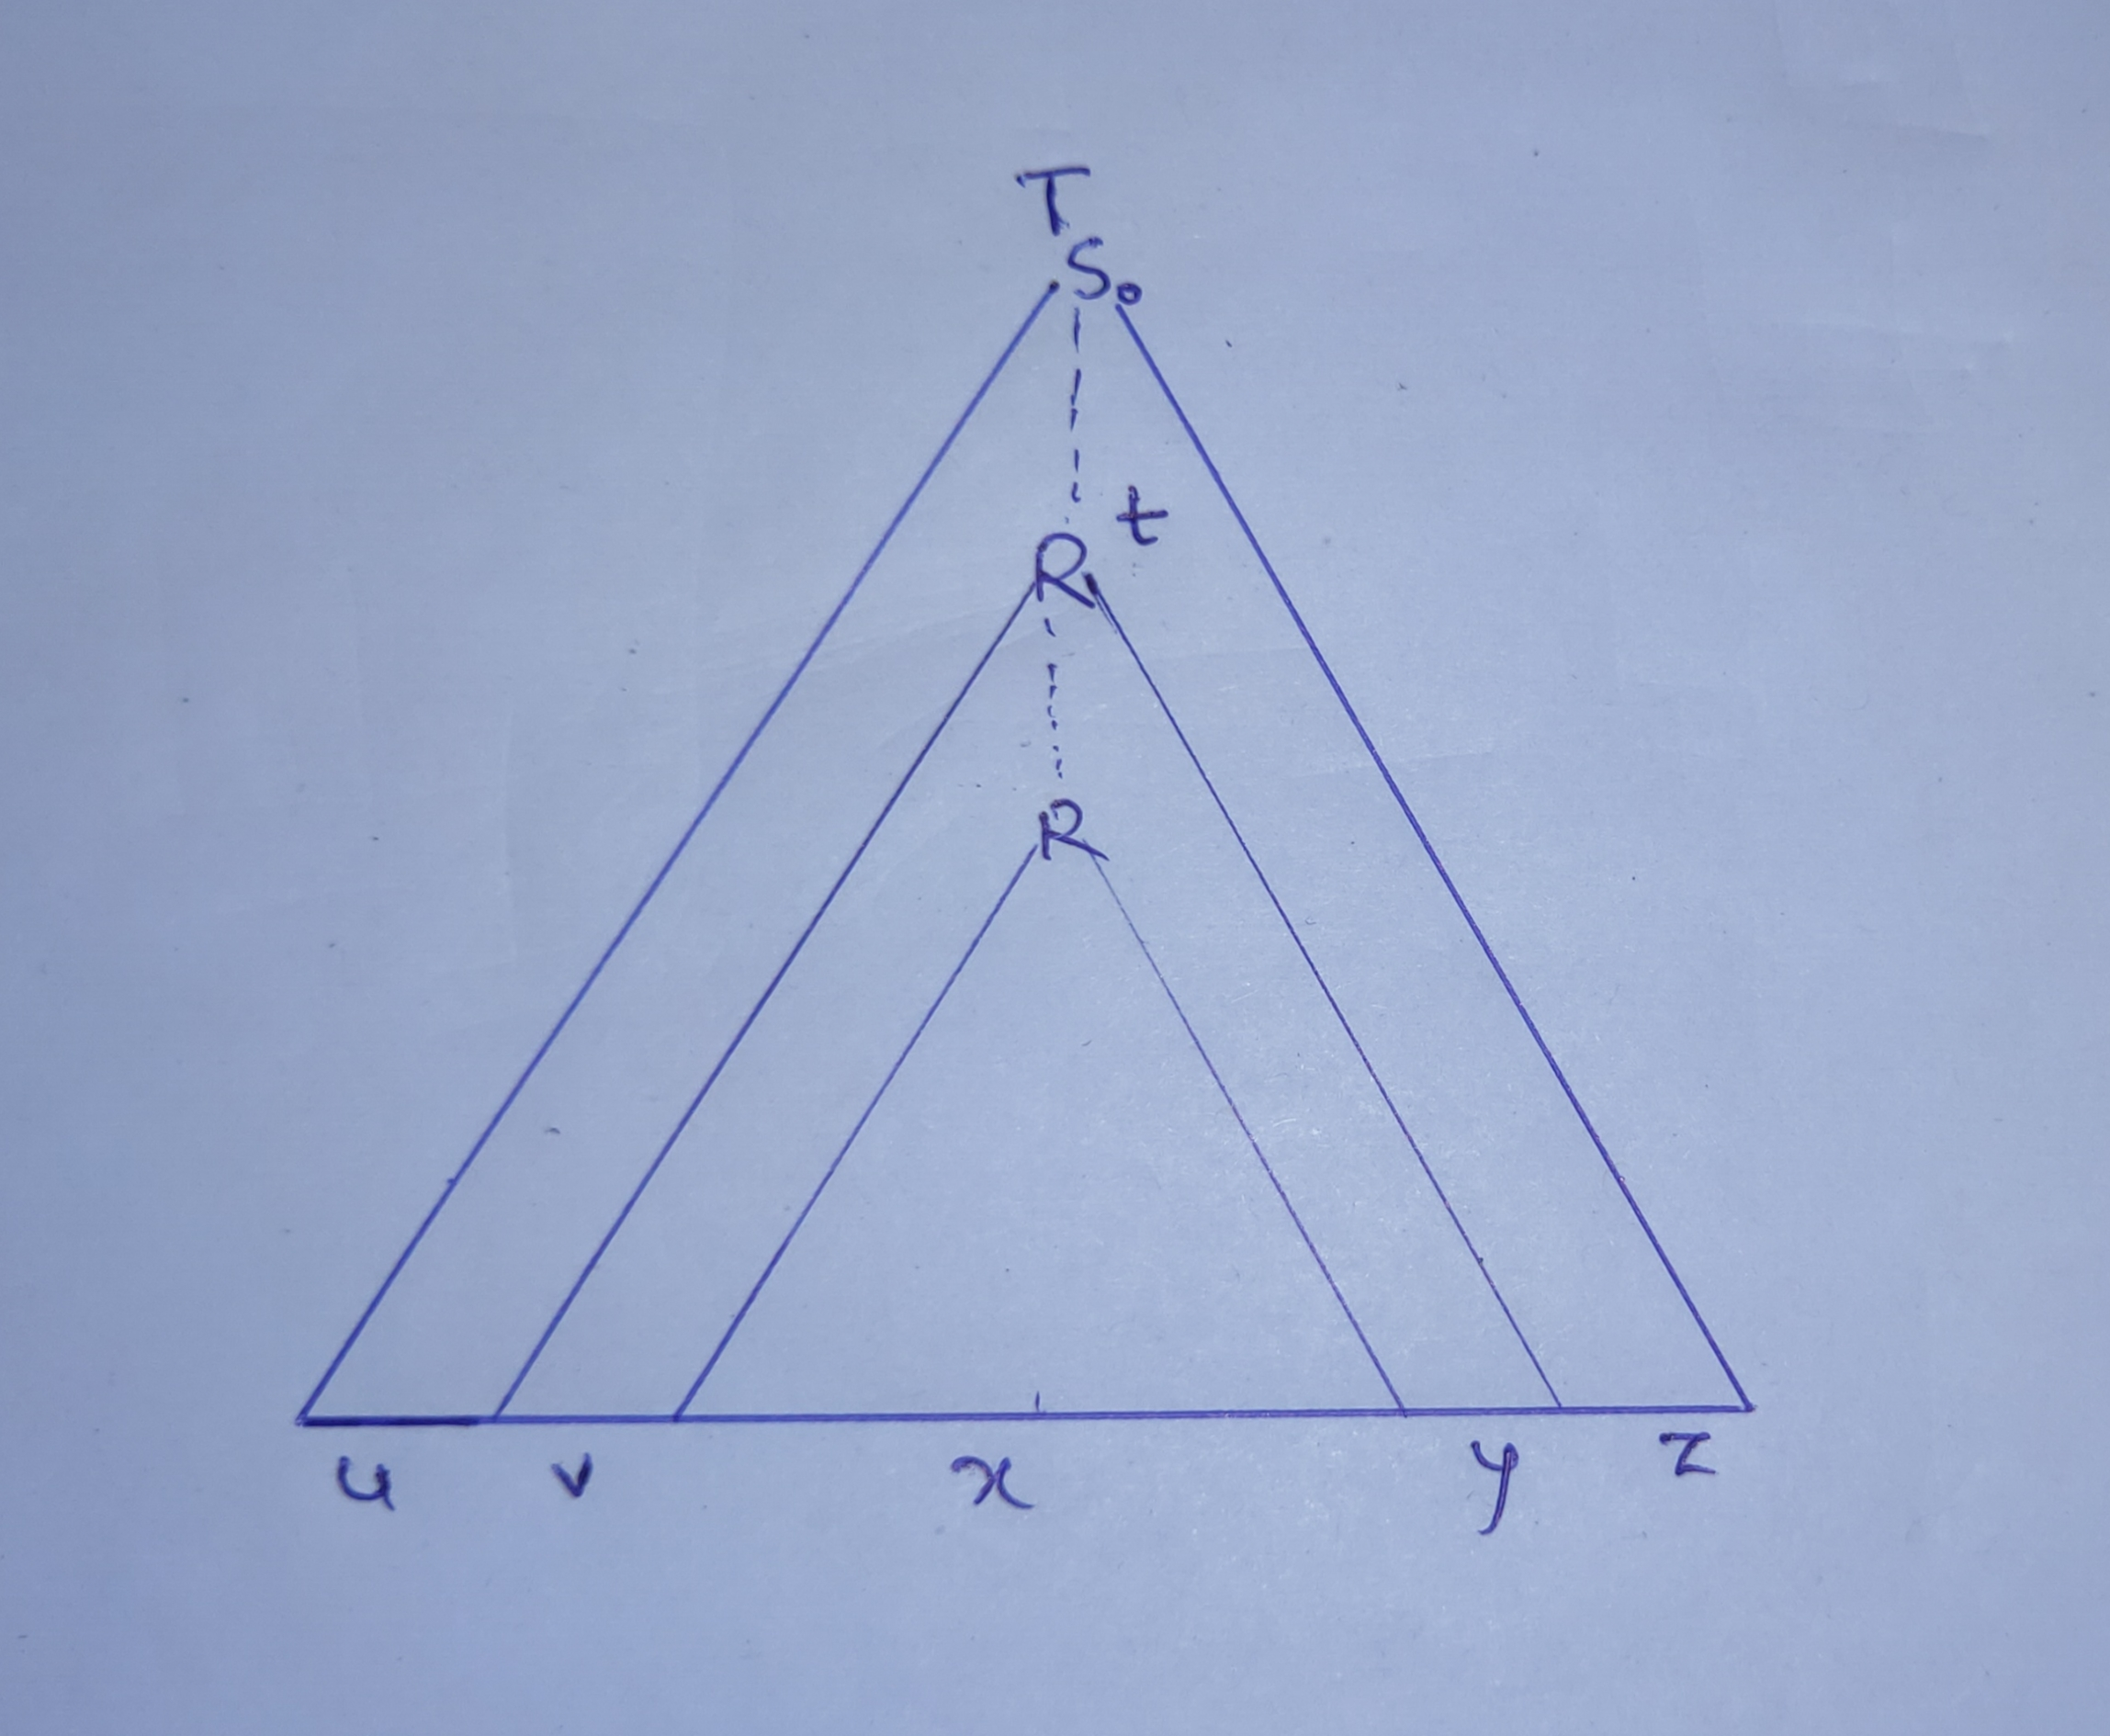
\includegraphics[width=0.5\linewidth]{graph/1.jpg}
    \caption{}
    \label{fig:7}
    \end{figure*}
    
    If either of v and y is equal to $\epsilon$ then one the child of R should be R as shown in Figure 4. But this is not the case because R is repeating thrice in the path and if we take first R and last R for our construction then the child of R can not be R. So, $v \neq \epsilon$ and  $y \neq \epsilon$ for the parse tree T.
    \begin{figure*}[!htb]
    \centering
    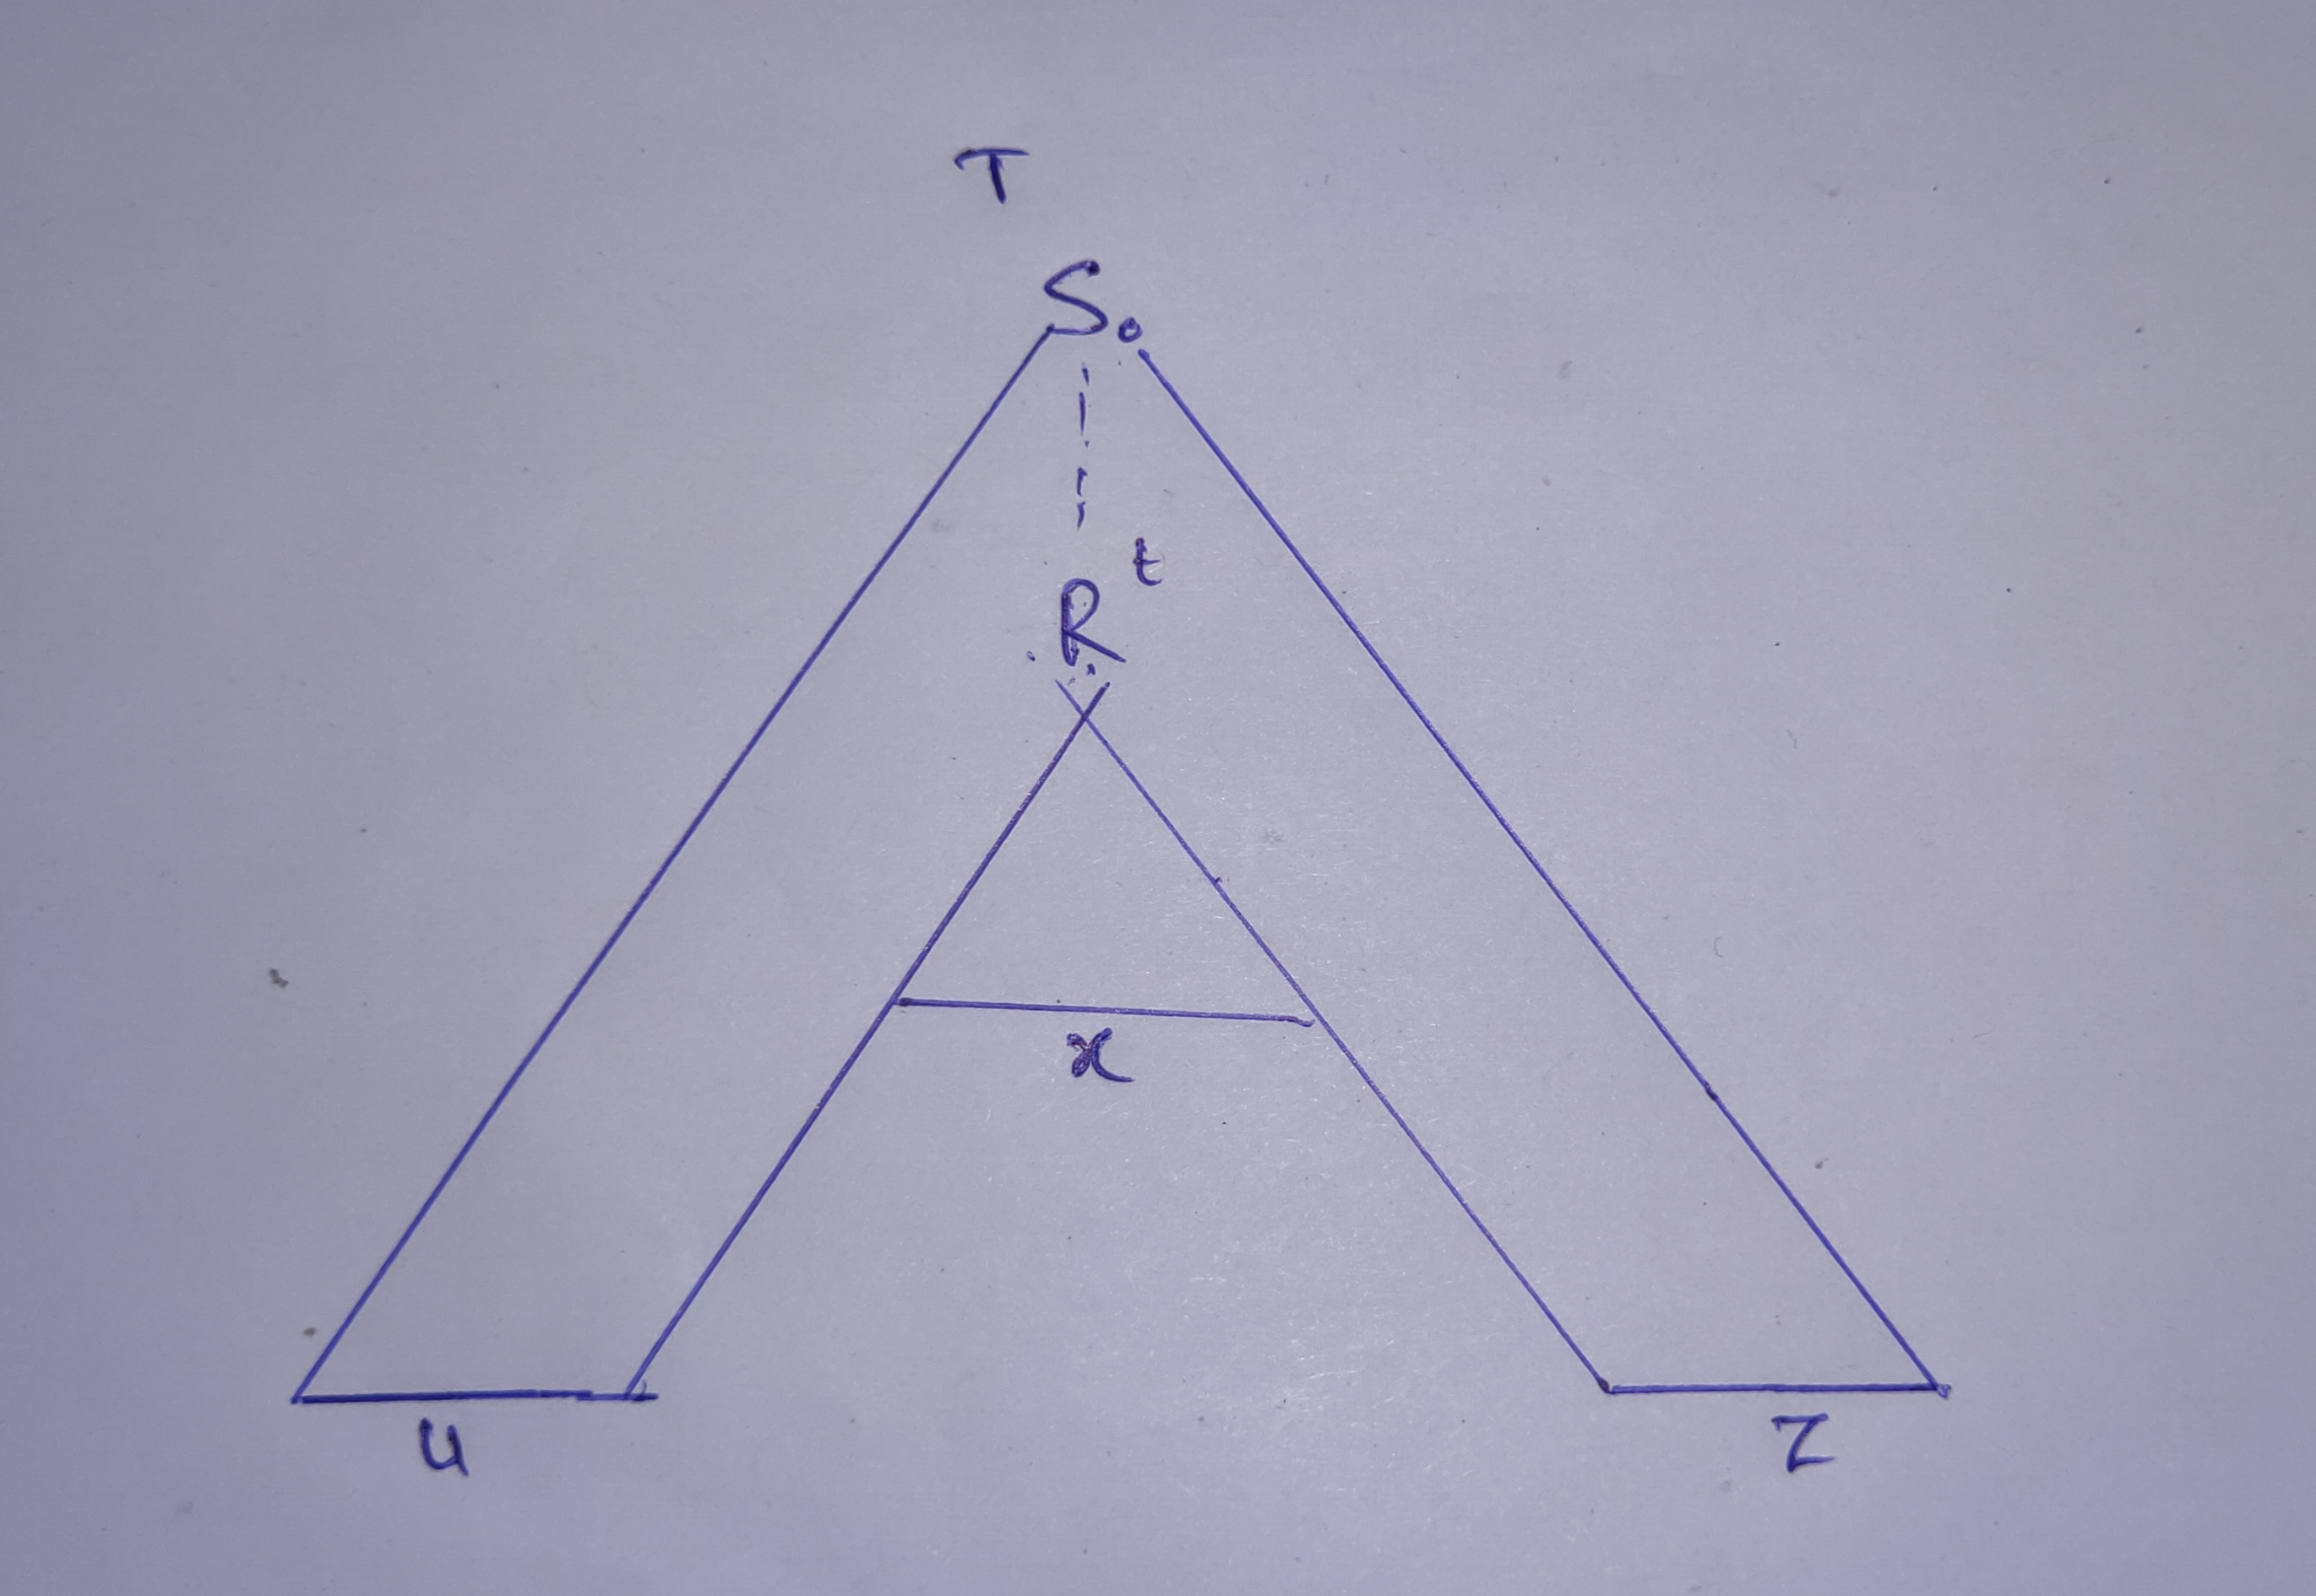
\includegraphics[width=0.5\linewidth]{graph/2.jpg}
    \caption{}
    \label{fig:6}
    \end{figure*}
    \\\\
    Let R be the the lowest thrice repeating non-terminal. Then depth of the sub-tree t can be at most $2 \vert V \vert + 1$ because if the depth is more than $2 \vert V \vert + 1$ then there must be another non-terminal which will repeat thrice in the sub-tree t by pigeon hole principle. This contradicts our assumption that R is the lowest thrice repeating non-terminal. Hence, depth $\leq$ $2 \vert V \vert + 1$ $\Rightarrow \vert vxy \vert \leq k$.  
    \begin{figure*}[!htb]
    \centering
    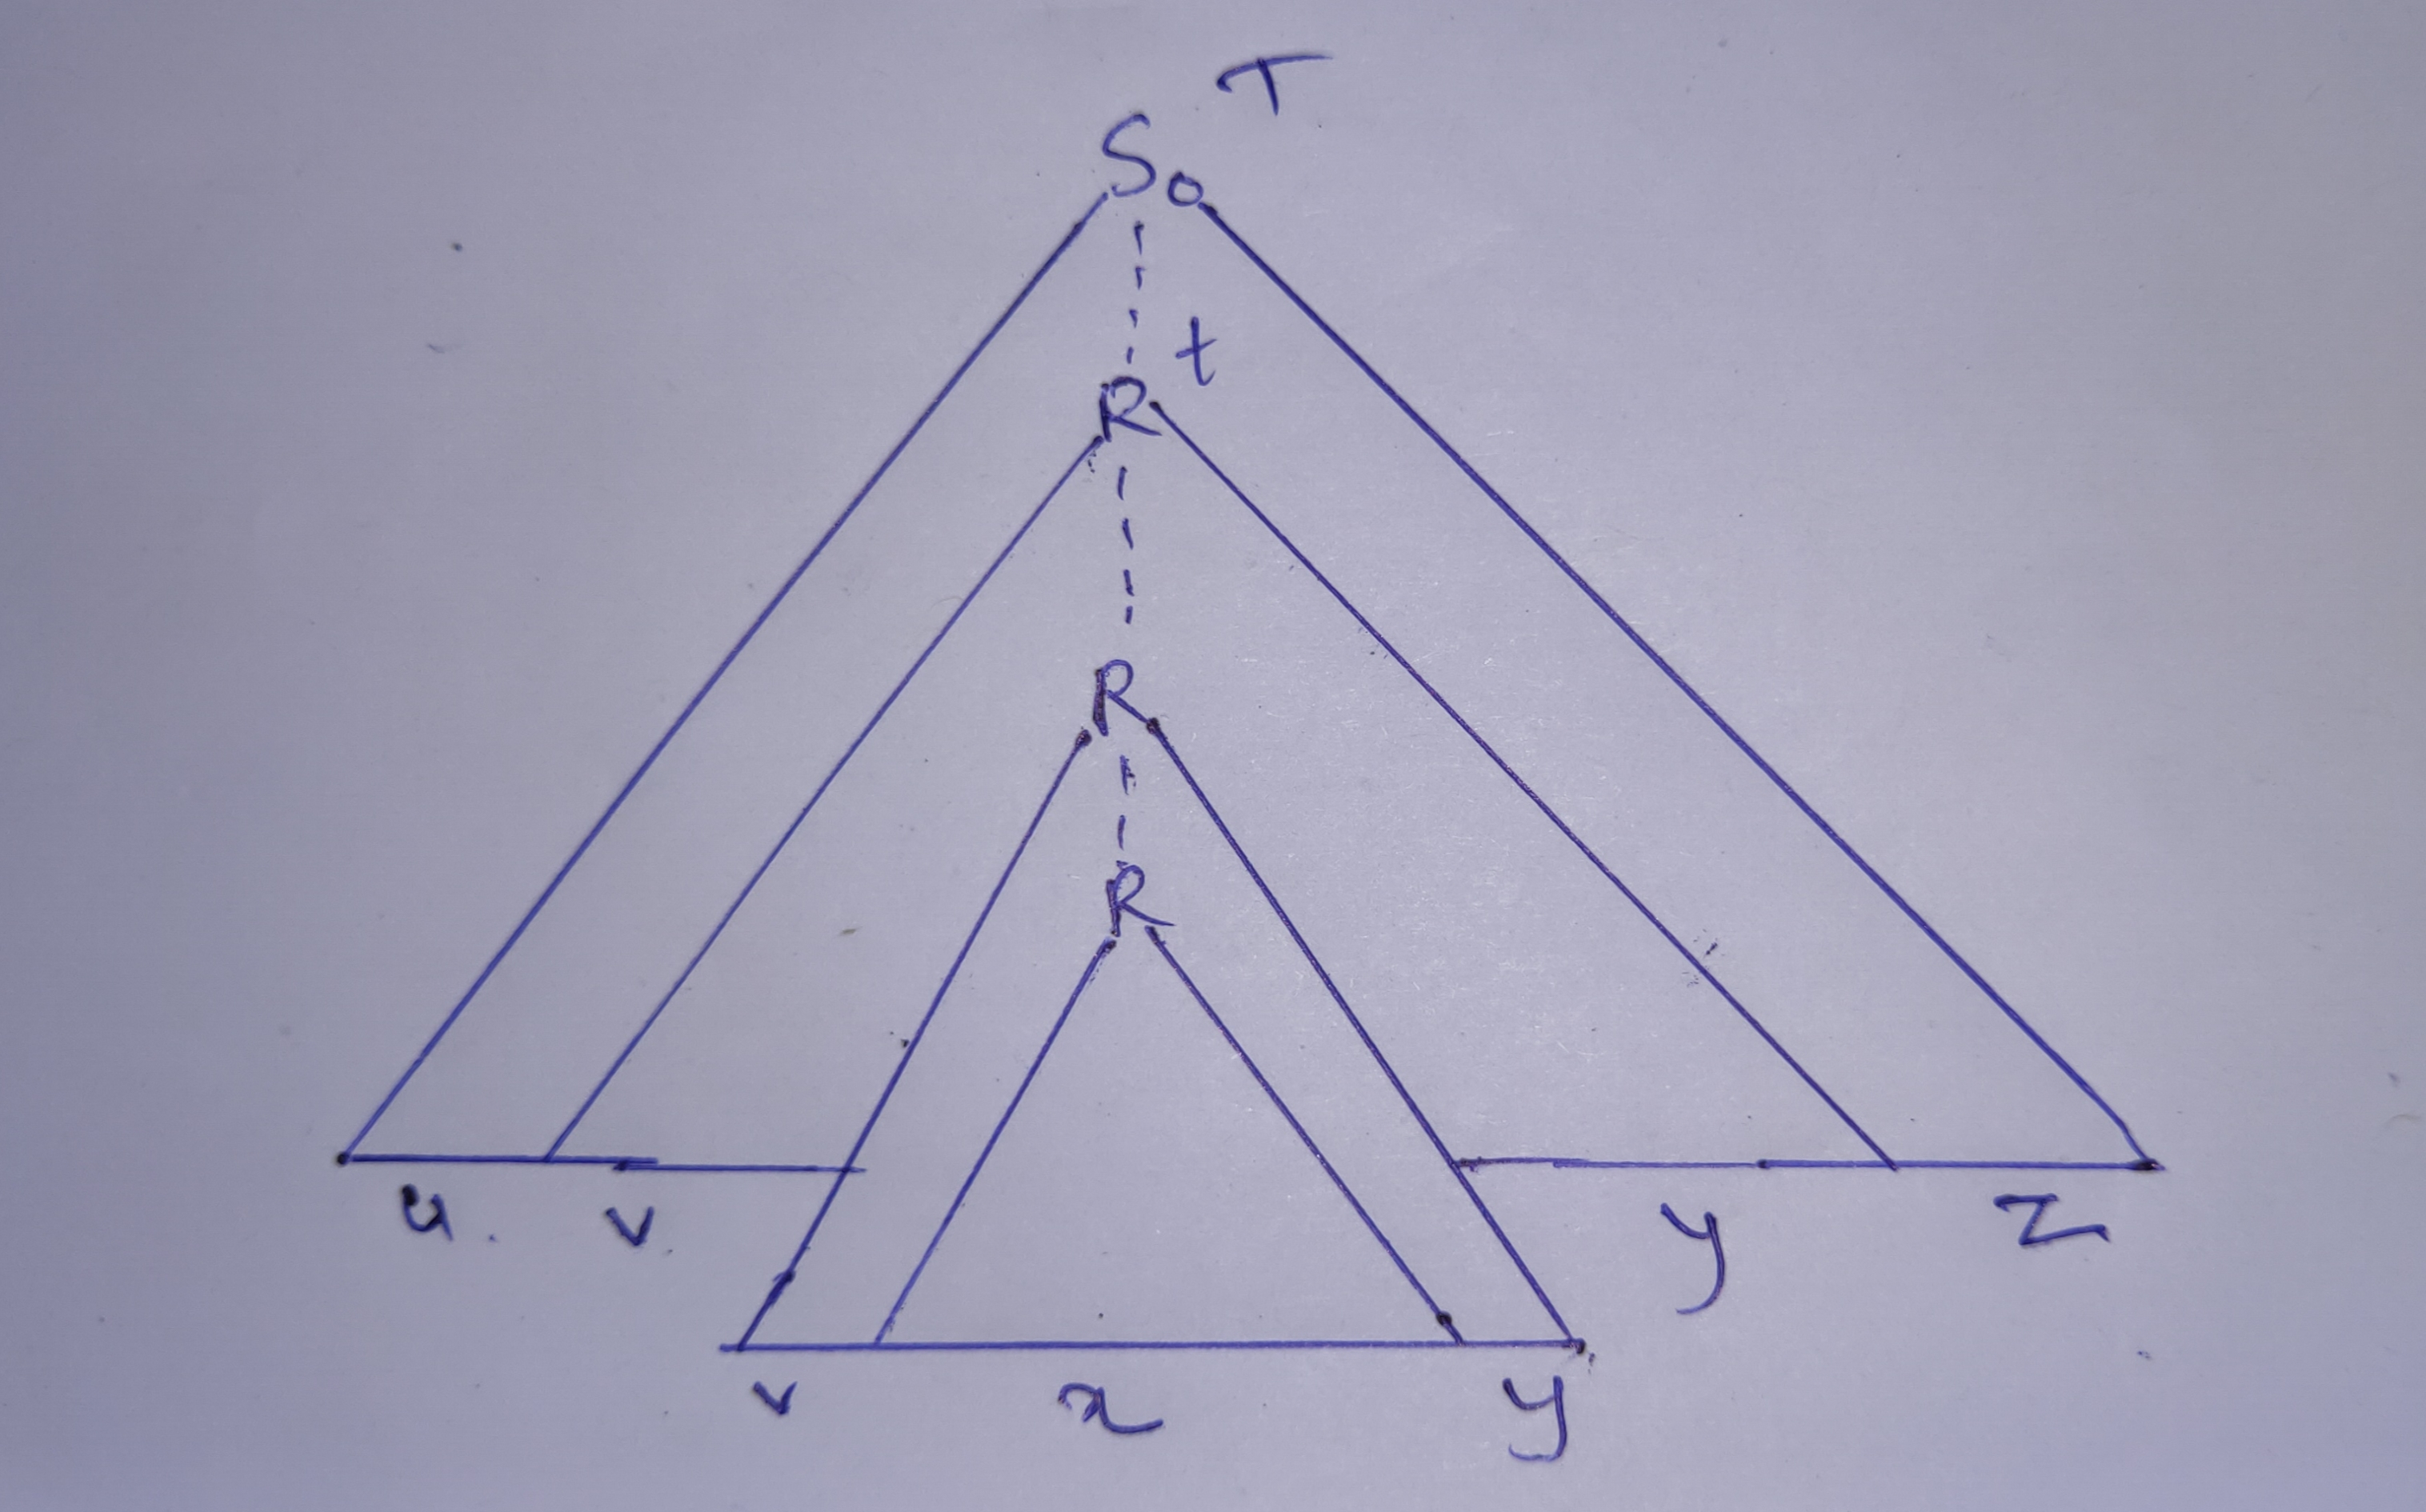
\includegraphics[width=0.5\linewidth]{graph/3.jpg}
    \caption{}
    \label{fig:6}
    \end{figure*}

    \begin{figure*}[!htb]
    \centering
    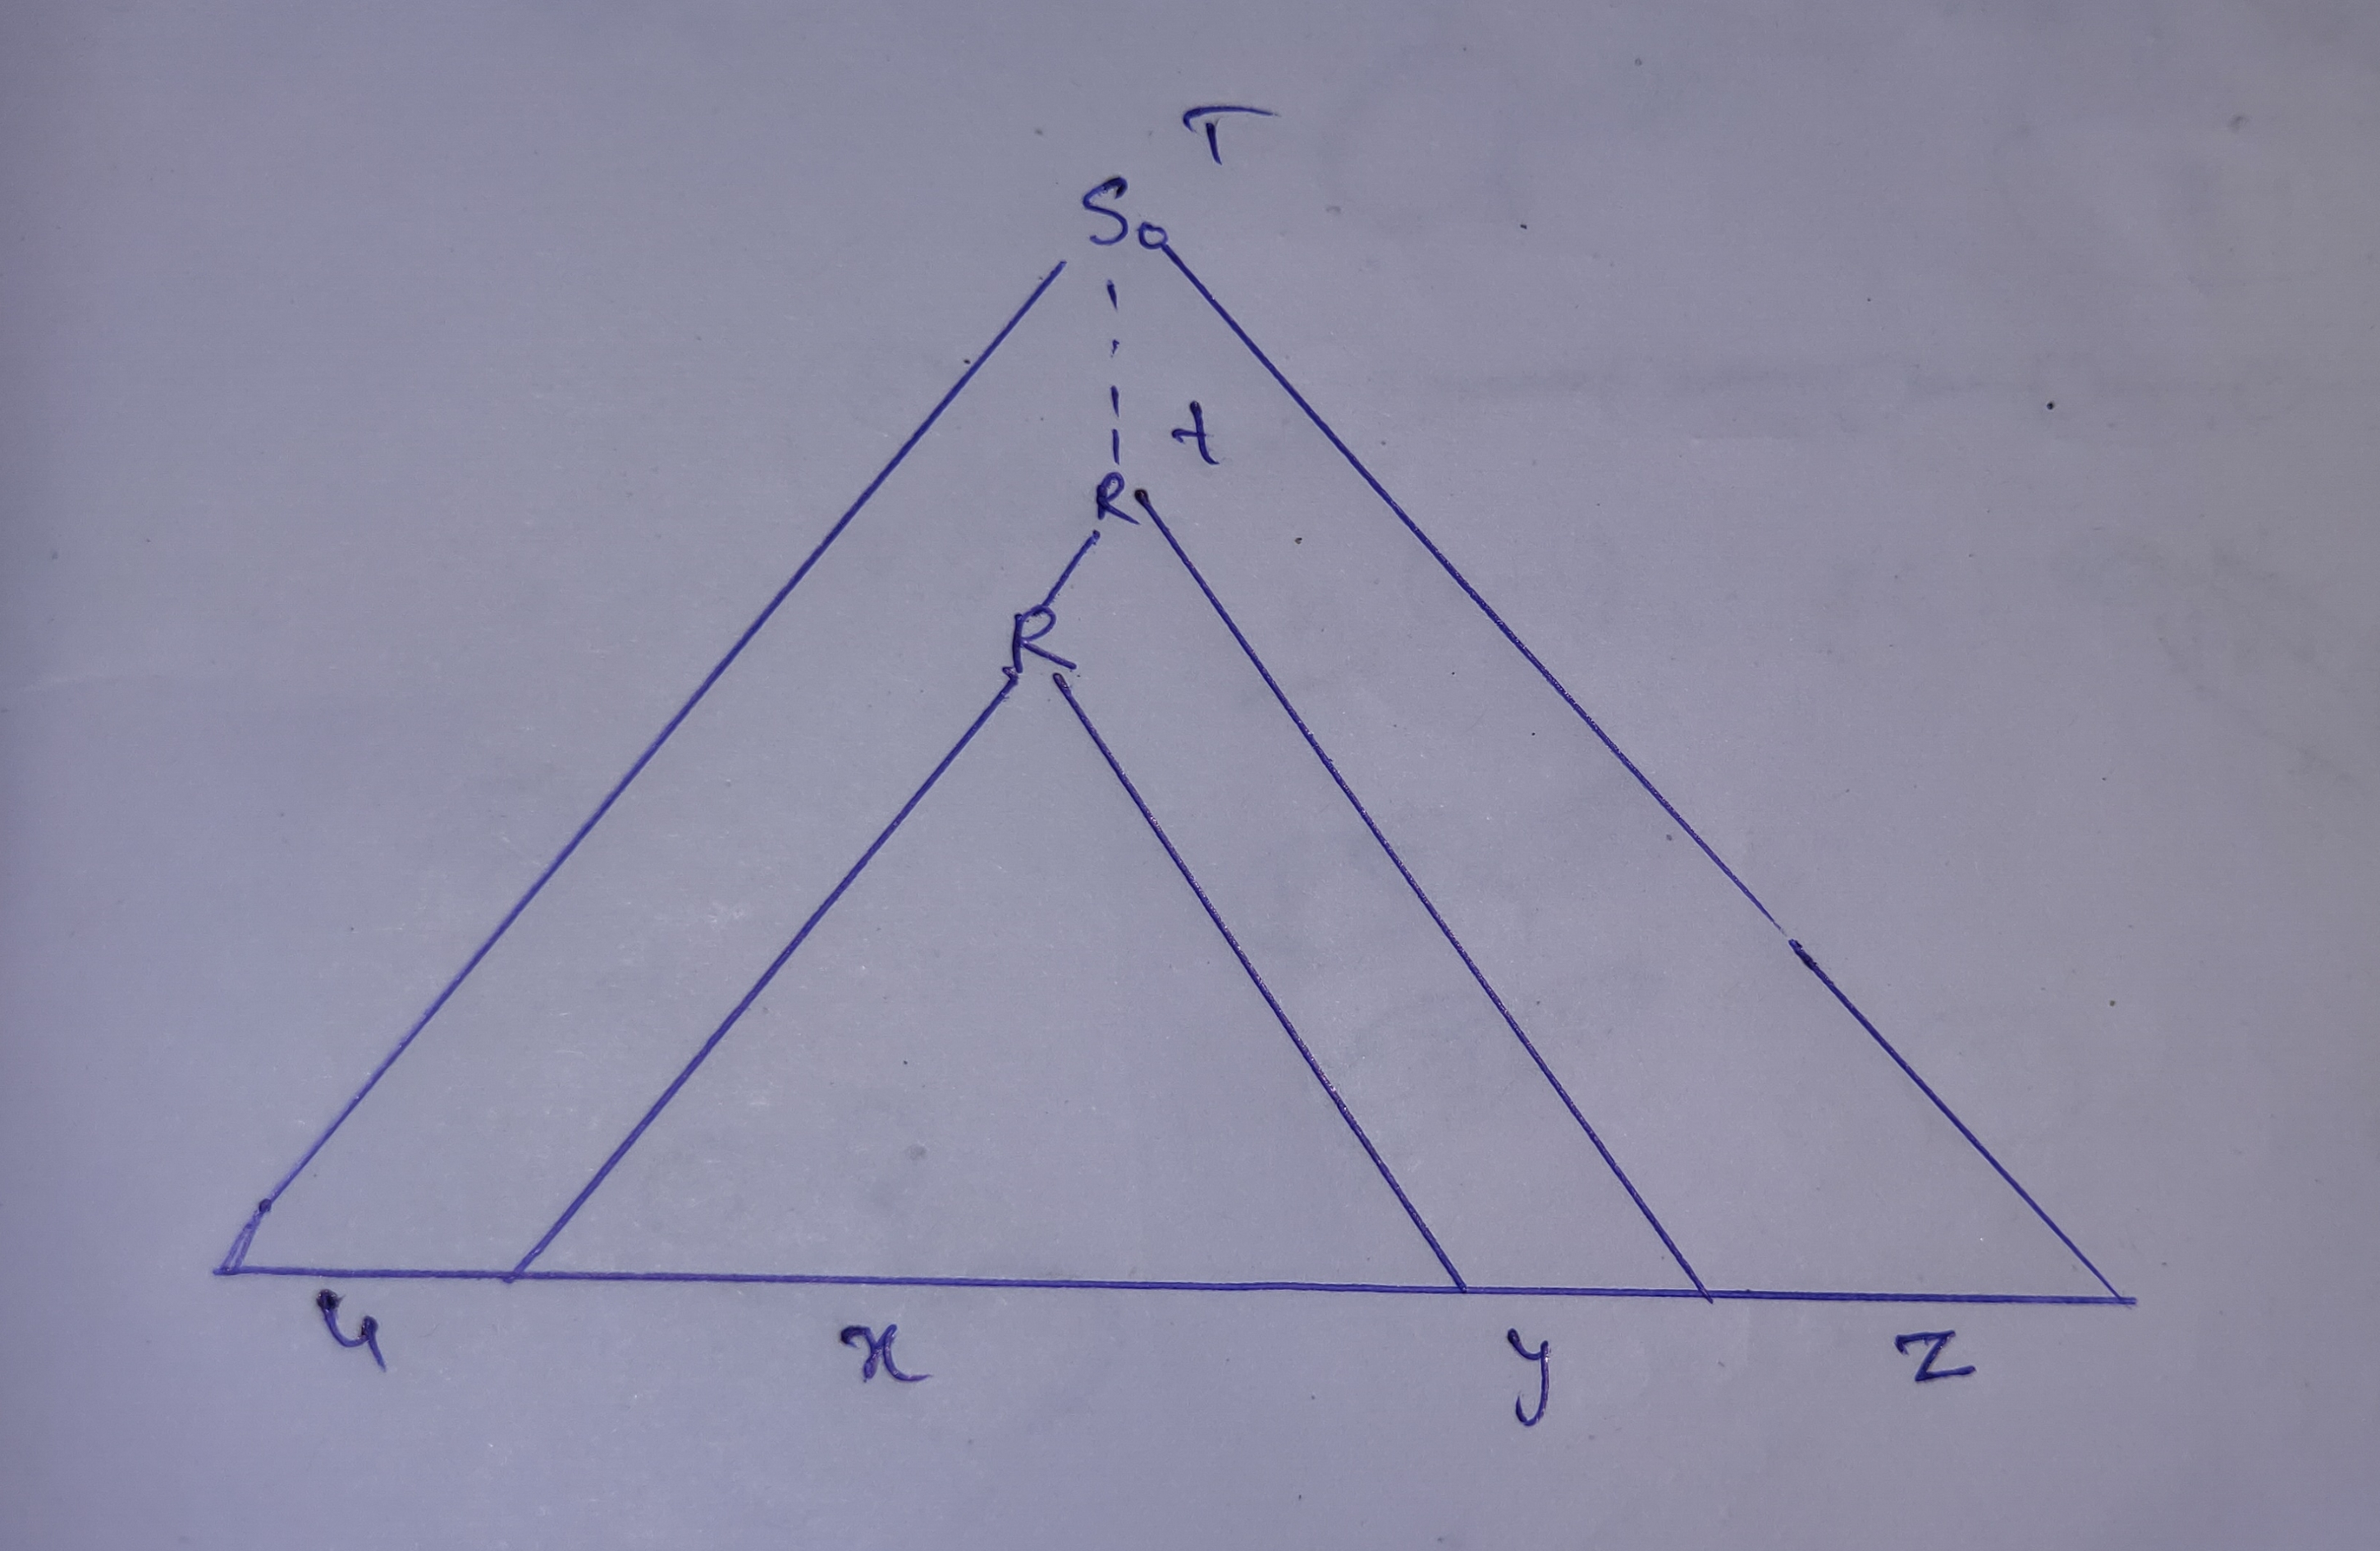
\includegraphics[width=0.5\linewidth]{graph/4.jpg}
    \caption{}
    \label{fig:6}
    \end{figure*}

    
	\algrule
	\clearpage
	
	\item Give an example of a language that is not a CFL but nevertheless acts like a CFL in the pumping lemma for CFL (Recall we saw such an example in class while studying pumping lemma for regular languages)
	
	\textbf{Solution:}\\
    Let us consider a language L = A $\cup$ B over $\Sigma = \{0,1,2,3\} $ where A = \{$01^n2^n3^n \vert  n \geq 1$ \}  and B = \{$0^it \vert t = \{1, 2, 3\}^* \text{and i} \neq 1$\}.\\ We know A is not a CFL as it does not satisfy the condition of pumping lemma similarly as shown in the class for $0^n1^n2^n$. So, L is also not a CFL as it is union of A and B. But if choose a pumping length, p $\geq$ 2 lets say p = 4 then,\\
    Case 1: If a string s $= 01^n2^n3^n$ is selected from A. We can pump first symbol of s which is 0 by taking u = $\epsilon, v = 0$ and remaining part of s as  wxy. The resulting string will stay in language B because it will be of the form $0^it$ if i $\neq$ 1 and remain in A if i = 1 which implies resulting string is also in language L. \\
    Case 2: If a string s $= 0^it $ is selected from B then we can pump first two symbols of s which is 00. The resulting string will be element of language B as B is CFL and satisfy pumping lemma which implies resulting string is also in language L.\\
    We can say that language L is satisfying pumping lemma conditions. \\\\
    Hence, from above it is shown that a non-CFL language L can acts like a CFL in the pumping lemma for CFL. 
	\algrule
\end{enumerate}


\end{document}
